%人間はロボットと同じ速度で動く


%本研究では,スーパーバイザの計算結果から,最適なふるまいを選び出す.
%全エージェントを同時に動いたとする.
%人間の安全を保障するため,最後に人間の行動を決定する.
%

\chapter{Human-in-the-loopにおける人間の安全性を確保する方法}\label{chap:method}

この章では,人間を考えた倉庫の中で人間の安全性を確保するためにどう制御するかという問題に対しての2つの方法を提案する.人間の普段の作業場所をスタート地点といい,トラブルが発生した場所,もしくはロボットに協力するために向かうロボットとの合流地点を目的地,そして人間が最終的に戻りたい場所をゴール地点とよぶこととする.
% トラブルなどを処理し終わった人間がそれまで行っていた作業に戻る場合,スタート地点とゴール地点が同じ地点になる.

\section{方法1}
1つ目の方法は,人間が使う通路上(スタート地点から目的地に向かうまでの経路と目的地からゴール地点に向かうまでの経路)をロボットに使わせないという考え方で制御を行う.人間が通る可能性のある通路についてロボットを完全に通行止めにする(図\ref{fig:area}).図の赤い部分がロボットの進入禁止エリアである.

\begin{figure}[h]
    \centering
    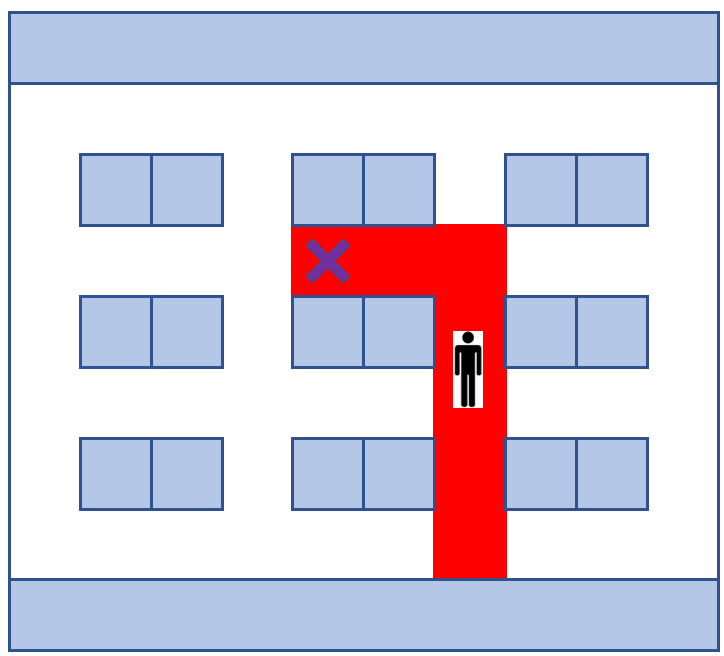
\includegraphics[scale=0.3]{figures/4_area.png}
    \caption{ロボットの進入禁止エリア}
    \label{fig:area}
\end{figure}

これを実現する具体的な方法は,不可制御事象をもちいて人間の行動を定義する方法である.行動すべてを不可制御事象で定義するということは,スーパーバイザからみて,人間の行動がいつ発生するかわからない,かつ発生を禁止することができない. 
\ref{sec:design_robot}節のとおり,倉庫内を移動しているロボットはスーパーバイザ制御理論でいう可制御事象で定義されており,指示を出すことができる制御対象である.それに対して人間は制御対象ではない.

例えば,ロボットに対しては「特定の場所で方向転換し,あるタイミングで,決まった速度で移動する」というように精密に指示することが可能だが,人間はロボットのように厳密に制御できるわけではなく,本人の意思によっても行動する.したがって,人間を制御するのではなく,制御対象ではないとするのが自然である.

ロボット同士の制御であれば,制御要求を満たさない行動,つまり衝突してしまう行動やブロッキング状態になってしまう行動を直前で禁止することができた.しかし,不可制御事象で定義された人間に対しては,スーパーバイザは制御要求を満たさない行動を禁止できない.また,人間の行動のタイミングもコントロールするのが不可能である.ロボットが人間の経路上に存在していると,連続して何回も人間が行動し続けた場合,衝突することになり制御要求を満たさない.このような理由で人間の経路はロボットから見て障害物のように認識される.
これを踏まえて,スーパーバイザが計算される.

この計算結果として,人間が安全な場所に到着するまで,人間の経路上にロボットを侵入させないというスーパーバイザが得られる.

% なんか書く.スーパーバイザ作る具体的な手順とか?

言い換えれば,人間のスタート地点から,トラブルが発生した場所や協力が必要なロボットとの合流地点までの経路を予約し,予約された通路をロボットから見て通行止めとすることで,人間の経路上には完全に立ち入らせず安全を確保する方法である.


\section{方法2}
2つ目の方法は,人間のいる位置を重視して,人間の周りだけにロボットの進入禁止エリアを定めるというものである.
1つ目の方法は,ロボットの進入禁止エリアを静的に定めていたのに対し,2つ目の方法では動的に変化する.

衝突回避の制御について,ロボット同士の場合は,どちらかのロボットの進行方向に別のロボットがいるときに行動を禁止している.これが人間とロボットの場合,人間の前に来てからロボットの行動を禁止するのでは,人間の恐怖心をあおるだけでなく,万が一エラーが起こることも考慮に入れると事故のもとになるという理由から,ロボットと人間の間に一定の距離を設ける必要性がある. 

また,そのロボットと人間が安全を確保するために最低限離れていなければならない距離(最小安全隔離距離)を任意に決められるように変数で扱うことにより汎用性を高める.ロボットの移動速度が大きければ制動距離のことを考慮して最小安全隔離距離を大きくとり,逆に移動速度が小さければ最小安全隔離距離も小さくするというように,最小安全隔離距離を変数とし,変更可能にすることにより様々なスペックのロボットに対応することができる.また,倉庫の規模によって変更することもできる.

具体的な方法としては,制御要求を拡張することで実現する.ロボットだけを制御するとき,制御要求は衝突回避のため,同じ瞬間に同じ位置に2つ以上のエージェントが存在する状態を排斥していた.それに対し提案する方法では,最小安全隔離距離を1マスとおいた場合,図\ref{fig:d=1}のように制御要求を人間を中心としてロボットが前後左右のマスにいる状態にまで拡張させる.また,最小安全隔離距離を2,3とおいた場合,それぞれ図\ref{fig:d=2},\ref{fig:d=3}のように進入禁止エリアを設定する.基本的に,ロボットが通路もしくは棚にいるときに接近を禁止する.ロボットが倉庫の待機場所もしくは搬出場所にいるときは距離をとる必要がないので進入禁止エリアに指定していない.

%この方法を使った場合,人間がすぐにはたどり着かない場所,つまり人間の安全が十分に確保されている場所はロボットも通ることができる.

\begin{figure}[h]
    \centering
    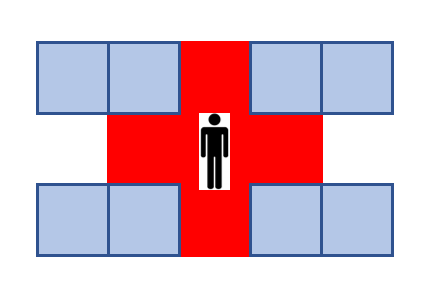
\includegraphics[scale=0.5]{figures/4_d=1.png}
    \caption{最小安全隔離距離 $d=1$}
    \label{fig:d=1}
\end{figure}

\begin{figure}[h]
    \centering
    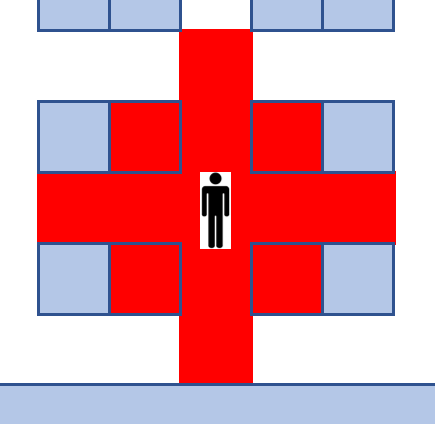
\includegraphics[scale=0.5]{figures/4_d=2.png}
    \caption{最小安全隔離距離 $d=2$}
    \label{fig:d=2}
\end{figure}

\begin{figure}[h]
    \centering
    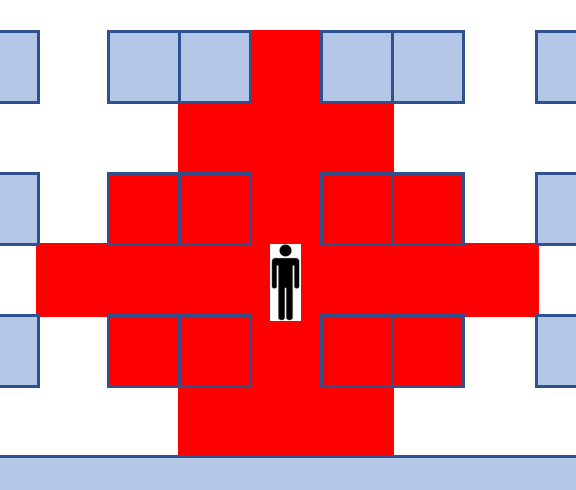
\includegraphics[scale=0.5]{figures/4_d=3.png}
    \caption{最小安全隔離距離 $d=3$}
    \label{fig:d=3}
\end{figure}


\ref{sec:design_sup}節の手順で計算を行うと,ロボットと人間がとり得るデータで制御要求を満たす状態遷移のすべてを網羅したスーパーバイザが出力される.そのスーパーバイザの状態遷移のうち,初期状態からどのようなふるまいで受理状態までの到達するのか選択する必要がある.すべてのエージェントが1回行動するもしくは行動しない一連の事象列の経過を単位時間(スーパーバイザの対象の数が$x$とすると\ $単位時間<x遷移$)とする.ロボットのみの制御を行う場合,スーパーバイザの初期状態から受理状態までかかる時間が最小のものを選ぶことで最も効率の良いタスクの処理といえる.しかし,人間を含めた制御を行う場合,たとえタスクを完了させるまでの時間が短くても,安全性を考えると人間の行動を禁止してロボットを優先する制御をすべきではない. 

また,実用化する観点からみたとき,ロボットのコストと人間のコストを比べると,ロボットを導入して運用することについては,運用費に対する初期投資が大きく,人を雇用するのについては,雇う時間が長ければ長いほどコストがかかると推測される.つまり,ロボットは固定費,人間は変動費といったように大まかに考えることにする.人件費においてはコスト削減の余地があるという点においても,ロボットと人間どちらかの行動を禁止するとなったとき,人間の行動を優先して,倉庫内の移動時間を短くすることが重要である.


